\documentclass[12pt, centerh1]{article}
\textwidth=165mm \headheight=0mm \headsep=10mm \topmargin=-10mm
\textheight=230mm %\footskip=1.5cm
\oddsidemargin=0mm
\documentclass[12pt,letterpaper]{article}
\usepackage[margin=1in]{geometry}
\RequirePackage[colorlinks,citecolor=blue,urlcolor=blue]{hyperref}
\usepackage{amsmath, amssymb,natbib}
\usepackage[mathscr]{euscript}
\usepackage{mathrsfs}
\usepackage{graphicx,bm}
\usepackage{subfig}
\usepackage{color}
\usepackage{subcaption}
\usepackage{subcaption}
\usepackage[table]{xcolor}
\usepackage{longtable}
\usepackage{amsthm}
\usepackage[mathscr]{euscript}
\usepackage{relsize}
\newcolumntype{P}[1]{>{\centering\arraybackslash}p{#1}}
\usepackage{rotating}
\usepackage{eurosym}
\usepackage{colonequals}
\usepackage{bbm}
\usepackage{lscape}
\usepackage{amsmath}
\usepackage{makecell}
\newcommand{\squeezeup}{\vspace{-13.0mm}}
\newcommand{\squeezebit}{\vspace{-7.0mm}}


% ---------------------------------------

\title{Modelling Reactionary Military Expenditure \\between Nations}
\author{\qquad Bryce Koomans$^{1}$ \qquad\  Chukun Wang$^{2}$ \qquad\  Jack Longwell$^{2}$ \\ 
        \qquad\ Mark Eskandar$^{2}$ \qquad\ Matthew Lenko$^{2}$ \qquad\  Yan Ning Zhang$^{2}$ \\
\small $^1$DeGroote School of Business, McMaster University, Ontario, Canada.\\[-6pt]
\small $^2$Department of Mathematics \& Statistics, McMaster University, Ontario, Canada.\\[-6pt] 
}
\date{{\small December 14, 2020}}

\linespread{1.5}
\pdfminorversion=4

\begin{document}

\maketitle
\begin{abstract}
%Due to their inherent violent nature, military's across history have raised concern within nations and people alike. For all of their benefits, the armed forces can be costly, both to a country's funds and their people's psyche. Because of this, methods were created to explain how the expenditure of capital on raising an army will affect other nations. The Richardson model uses two equations representing the spending of two rival entities across time. There are several principal factors that the model accounts for, including fear, grievance, and fatigue. Within our report, we model the relation between the former Union of Soviet Socialist Republics (USSR) and the North Atlantic Treaty Organization (NATO), as well as the relation between the USSR and the United States of America. We also provide some insight into how the spending would have continued had the USSR not collapsed.

Due to their inherent violent nature, armed forces across history have raised concern within nations and people alike. For all of their benefits, the armed forces can be costly, both to a country's funds and their people's psyche. Because of this, methods were created to explain how a nation's expenditure on military ventures impacts another nation. Utilizing a simulation study, it is determined that the Richardson Model, accounting for all factors, produces an optimal fit to the Cold War expenditure data. Interpreting the data we find that a reduction in the United States military expenditure leads to decrease in the former Union of Soviet Socialist Republic's (USSR) military expenditure at the apex of the Cold War. It is inferred that a de-escalation of military expenditure by the United States would have had a larger impact on the pace of the arms race than a reduction by the North Atlantic Treaty Organization (NATO) would have had. 

\vspace{3mm}

\noindent\textbf{Keywords}: military expenditure; modelling; data; USSR; NATO; USA; differential equation, non-linear.
\end{abstract}

%----------------------

\section{Introduction}
Military forces harbour the power to spread peace and prosperity across the world \citep{rigby2006there}. As \cite{rigby2006there} and \cite{bellamy2009responsibility} detail, entities with military influence have the ability and responsibility to facilitating global humanitarian aid as well as liberate and protect global citizens; both of which are positive aspects of military use. However, nation's and international organizations such as the North Atlantic Treaty Organization (NATO) emphasizing military power across the world in the name of peace face risks and negative consequences \citep{rigby2006there}. In contrast with the military's ability to spread peace is the potential for reactionary conflict. An example of this cause-and-effect relationship between military powers is the potential for arms races.  Arms races, hereby defined as the competition between one or more entities to best each other's military might \citep{smith2020influence}, have historically led to instability and conflict as prominently exemplified in the escalation of World War I \citep{mahnken2016arms}. An infamous arms race: the Cold War, involved the United States and its allies in NATO continuously expanding their military armament at record costs \citep{10.2307/446958} to deter the USSR, which was also expanding its military power \citep{yost2010nato}, from exerting its military power. Exploring the United States and NATO's involvement in the Cold War, we seek to discover if the formation of NATO contributed to the increased military expenditures of the Cold War and whether it's disbandment could have stopped the arms race. For the intents and purposes of our inquiry, it is assumed that lower military expenditure implies more peaceful and normalized relations between foreign entities \citep{solarin2018determinants}.

Our inquiry is conducted utilizing the Richardson's Arms Race Model. The model, which was introduced by Lewis Fry Richardson in his 1960 work, \emph{Arms and Insecurity} \citep{smith2020influence}, models the relationship between nations using a system of differential equations \citep{mooney1999course}. Richardson's pair of differential equations are generalized as 
\begin{equation*}\label{NS}
    \frac{dx}{dt}= ay - cx + g_{xy} \quad ,\quad \frac{dy}{dt} = bx - dy + g_{yx}
\end{equation*}
The model approximates military expenditure using three different coefficients. The fear factors, which track the change in expenditure in response to the other nation's change in expenditure, fatigue factors which limit the total expenditure of the model, and constant grievance factors that track on-going quarrels between nations \citep{mooney1999course}. Most commonly Richardson's model is used to track military expenditure between competing nations \citep{smith2020influence}. However, the pair of differential equations have also been utilized to track the spending relationships between competing businesses \citep{chalikias2014implementation} and biological predator-prey models \citep{smith2020influence}. In our inquiry, the model is used in the traditional manner; modelling reactionary military expenditure between pairs of nations, with a specific application to NATO's influence on global relations. 

%----------------------

\section{Methodology}

\subsection{Data Processing}

The data sets used in our inquiry are acquired from Our World in Data's military spending research, which is compiles military expenditure data published by \emph{The Correlates of War Project} \citep{owidmilitaryspending}. The data assembled by Our World in Data categorizes the information by country name, year (reported annually from 1949 to 1989), and expenditure in billions of United States Dollars (USD) corrected for inflation to the year 2000.  The data is downloaded as a comma-separated values (.csv) file that is transformed to a text file (.txt). The text file is then loaded into Python \citep{10.5555/1593511} using the NumPy module's loadtxt feat \citep{2020NumPy-Array}. The data for our inquiry is then parsed by country's that are members of NATO. Each country's expenditure is only added to the NATO expenditure total after and including the year that the country joined the organization \citep{nato_2020}. Simultaneously, the United States and USSR's military expenditure is extracted with dates starting at the formation of NATO in 1949 \citep{nato_2020}. The scatter plot of processed data over time is available in the processed data plot appendix. 
\subsection{Richardson's Model}

For the purposes of our inquiry, the relationships between each entities military spending are represented using two systems of differential equations. First, the equations that model reactionary expenditure between NATO, $n$, and the Soviet Union, $s$, during the Cold War are
\begin{equation*}\label{NS}
    \frac{dn}{dt}= as - cn + g_{ns} \quad ,\quad \frac{ds}{dt} = bn - ds + g_{sn}
\end{equation*}
Second, the relationship between the United States, $u$, and the Soviet Union, $s$ are
\begin{equation*}\label{NS}
    \frac{du}{dt}= as - cu + g_{us} \quad ,\quad \frac{ds}{dt} = bu - ds + g_{su}
\end{equation*}
In both sets of differential equations, $a$ and $b$ are the fear factors between entities. Coefficients $c$ and $d$ are fatigue factors that limit the rate of growth of each differential equation. Finally, the coefficient $g_{ij}$ represents the grievance factor of country $i$ for country $j$. The grievance factor can be positive or negative based on the nation's relations \citep{mooney1999course}.

\subsection{Optimizing Model Coefficients}

Determining optimal model coefficients for the purposes of our inquiry were completed using non-linear optimization in Python \citep{10.5555/1593511}. Coefficient optimization is done through minimizing the sum of standard squared error (SSE) between both differential equations and their respective data points, which is evaluated as
\begin{equation*}\label{NS}
    SSE = \mathlarger{\mathlarger{\sum}}_{i=1}^{n}((x_i-\Bar{x})^2 + (y_i-\Bar{y})^2)
\end{equation*}
Where $x_i$ and $y_i$ are output values of each optimized differential equation and $\Bar{x}$ and $\Bar{y}$ are the averages of each set of outputs. Minimization of the SSE function is done using the minimize function of the optimize package of the SciPy module \citep{2020SciPy-NMeth}. 
\subsection{Plot Construction}

The graphing of our optimized Richardson Model differential equations is completed by integrating each system of differential equations. The differential equations are integrated using the odeint function of the integration package within the SciPy Python module \citep{2020SciPy-NMeth}. Each plot contains time, in units of years, on the x-axis and military expenditure, measured in tens of billions of US dollars adjusted to the year 2000, on the y-axis. All plots are constructed using the pyplot feature of the matplotlib package \citep{Hunter:2007}.

%----------------------

\section{Application}
%Any assumption? 
We begin by making and plotting models for both systems to fit our data by optimizing and solving for the coefficients. To accomplish our goal of investigating whether the Soviet Union’s response to NATO was greater than its response to the United States, we first need to find the best fitting model with the lowest cumulative SSE. 

% We performed the simulation study to model with different combinations of the coefficients, which are fear factors, fatigue factors and grievance factor. Then see how each factor influences the best prediction line of expenditure between the Soviet Union, NATO and the United States, and find the best fit model for the two systems.

% Then we are able to compare the reaction of the Soviet Union to the United State and NATO by predicting the trend of military expenditure in several years after 2007 for the two systems with the three-variable model.

\subsection{Simulation Study}
%If your model or problem set has parameters your change, this is where you would write about it. 
%Minimum 1 and a half pages. 

Determining the optimal combination of coefficients in the Richardson Model to best fit the military expenditure data is done using a simulation study. Using three distinct simulations, the model with the smallest sum of squared error is determined. 

The first simulation fits a model to the expenditure data using only the fear factors, $a$ and $b$. The two systems of differential equations and models are
\begin{equation*}\label{NS}
    \frac{dn}{dt}= as \quad ,\quad  \frac{ds}{dt} = bn 
\end{equation*}
\begin{equation*}\label{NS}
    \frac{du}{dt}= as \quad ,\quad \frac{ds}{dt} = bu 
\end{equation*}
%The resulting model fits using non-linear optimization are 
\squeezeup
\begin{figure}[htb!]
    \centering
    \subfloat{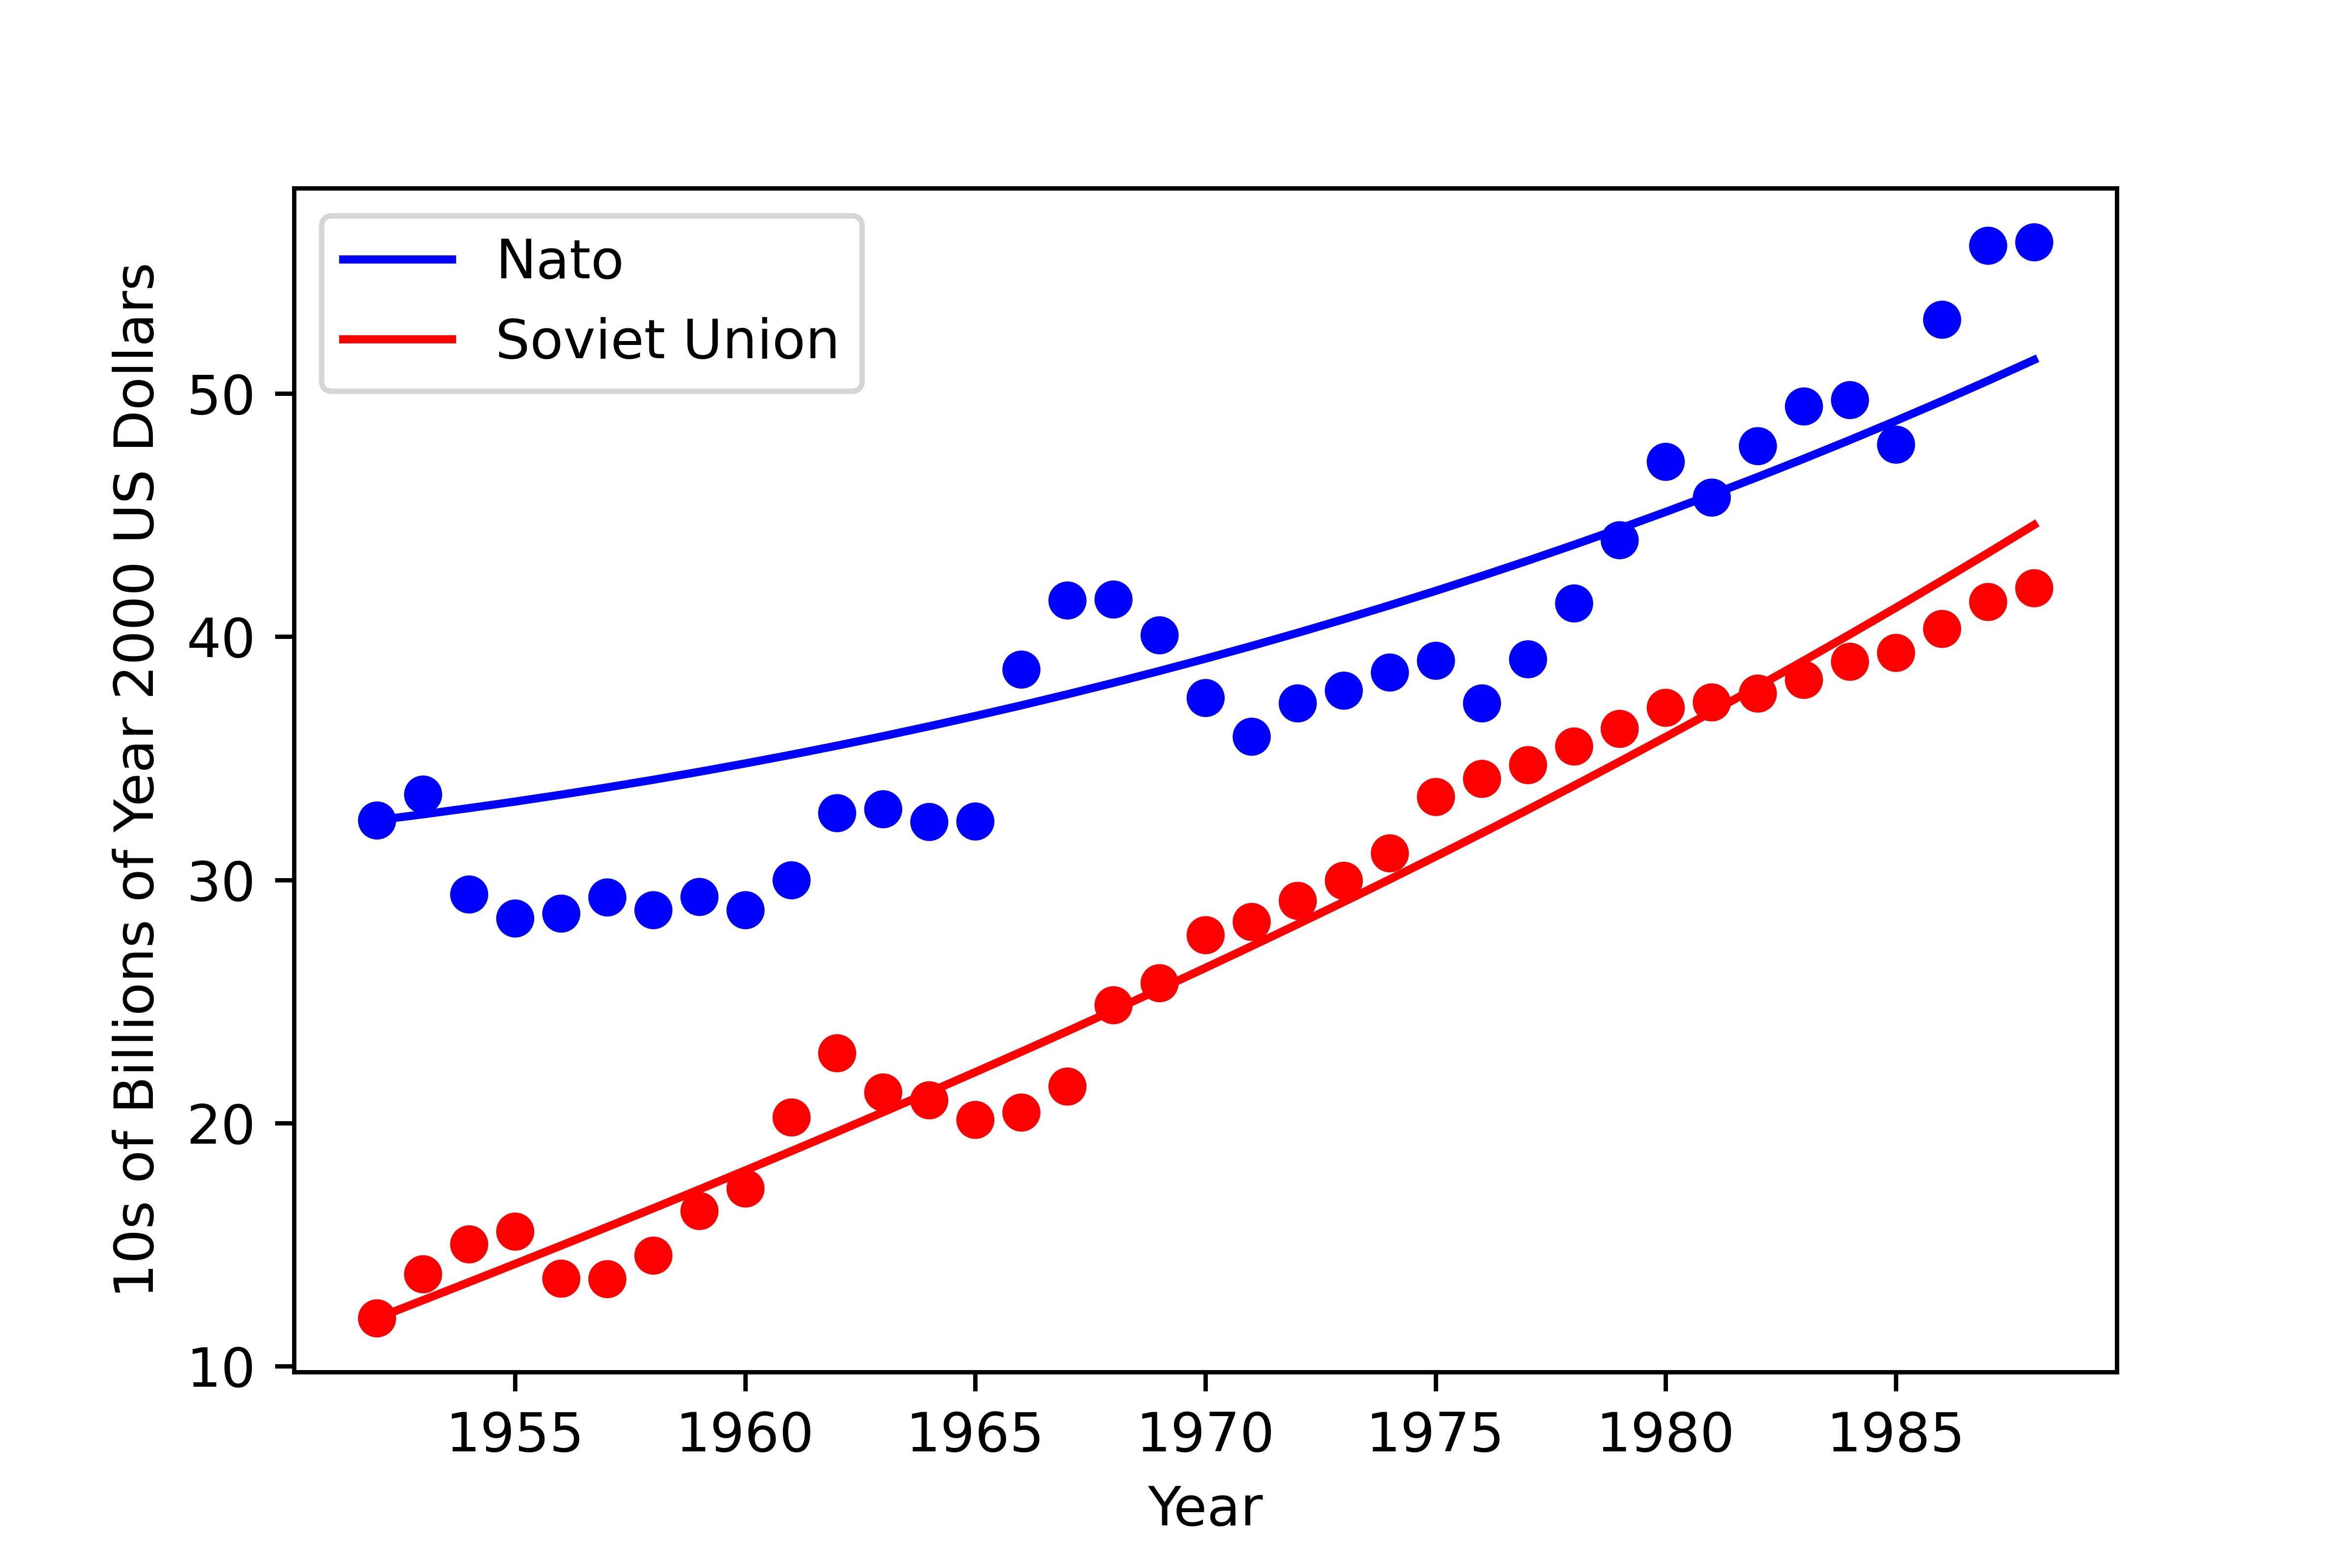
\includegraphics[width=8.25cm\textwidth]{NS1.png}\label{NS1}}
    \hfill
    \subfloat{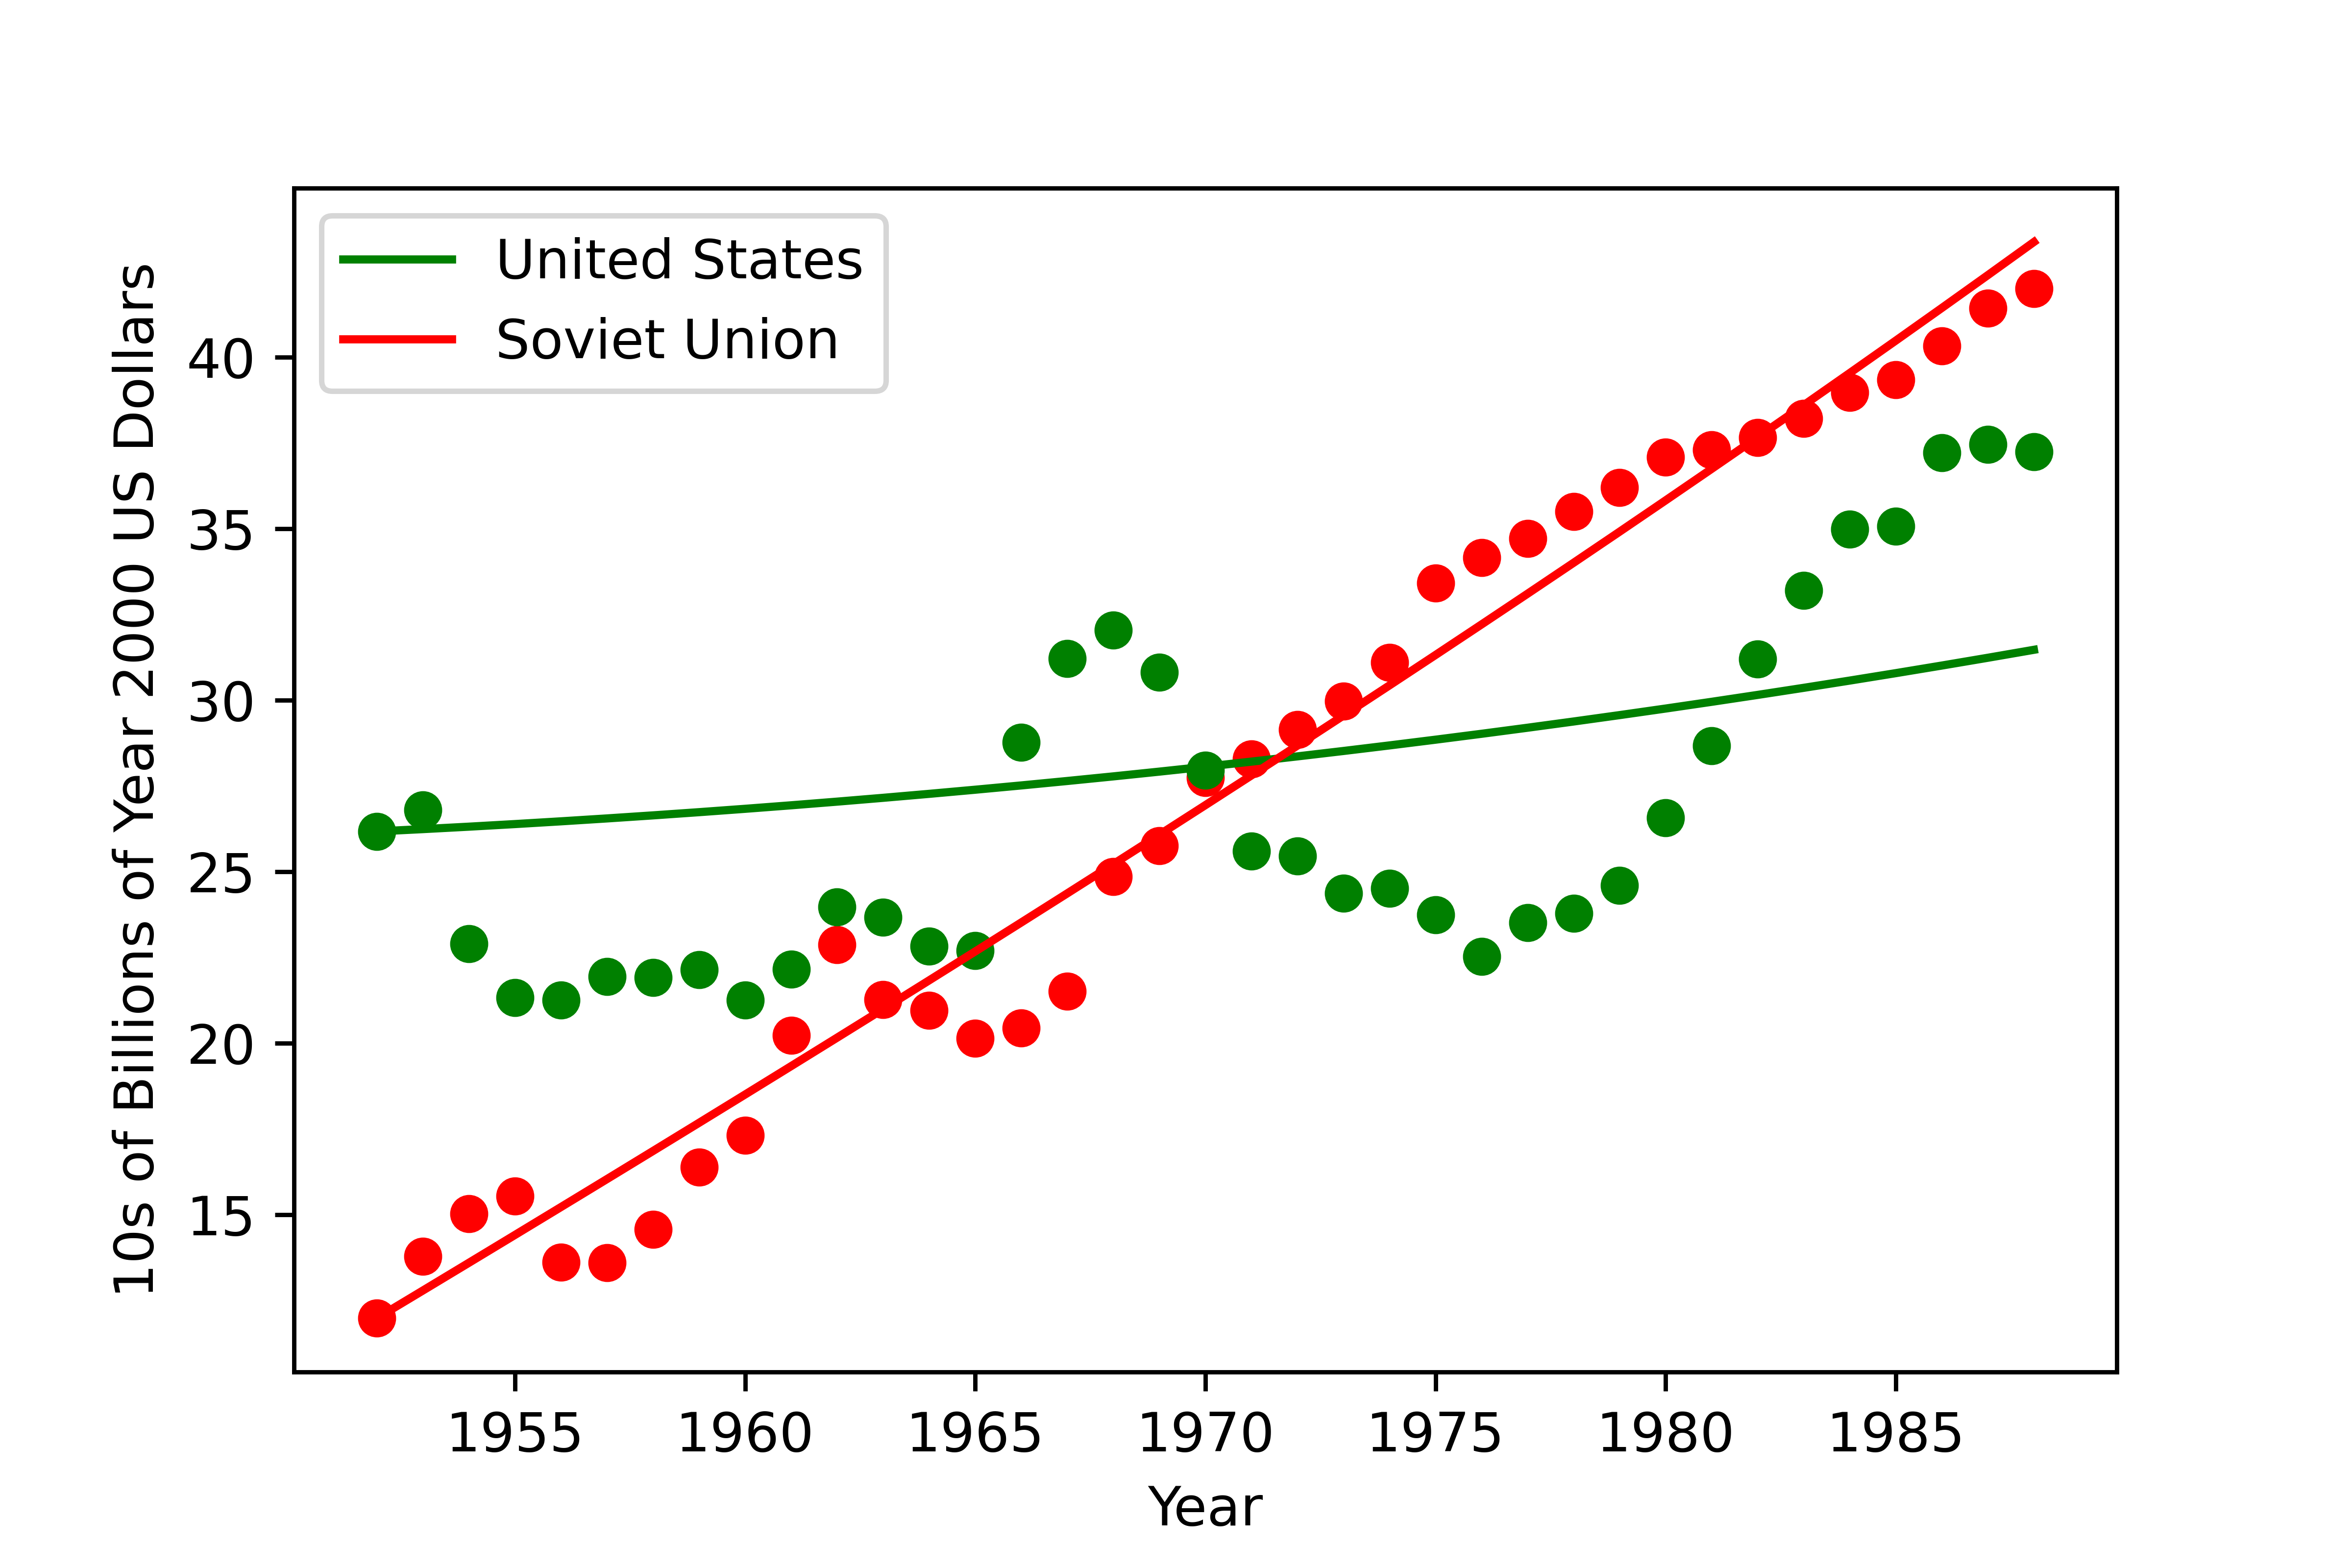
\includegraphics[width=8.25cm\textwidth]{US1.png}\label{US1}}
    \caption{One Variable Richardson Model Fit}
\end{figure}
\newpage
The second simulation fits a model using the fear factors, $a$ and $b$, as well as the fatigue factors, $c$ and $d$. The pair of differential equations and models are 
\begin{equation*}\label{NS}
    \frac{dn}{dt}= as - cn \quad ,\quad  \frac{ds}{dt} = bn - ds
\end{equation*}
\begin{equation*}\label{NS}
    \frac{du}{dt}= as -cu \quad ,\quad \frac{ds}{dt} = bu - ds
\end{equation*}
%The resulting models are
\squeezeup
\begin{figure}[htb!]
    \centering
    \subfloat{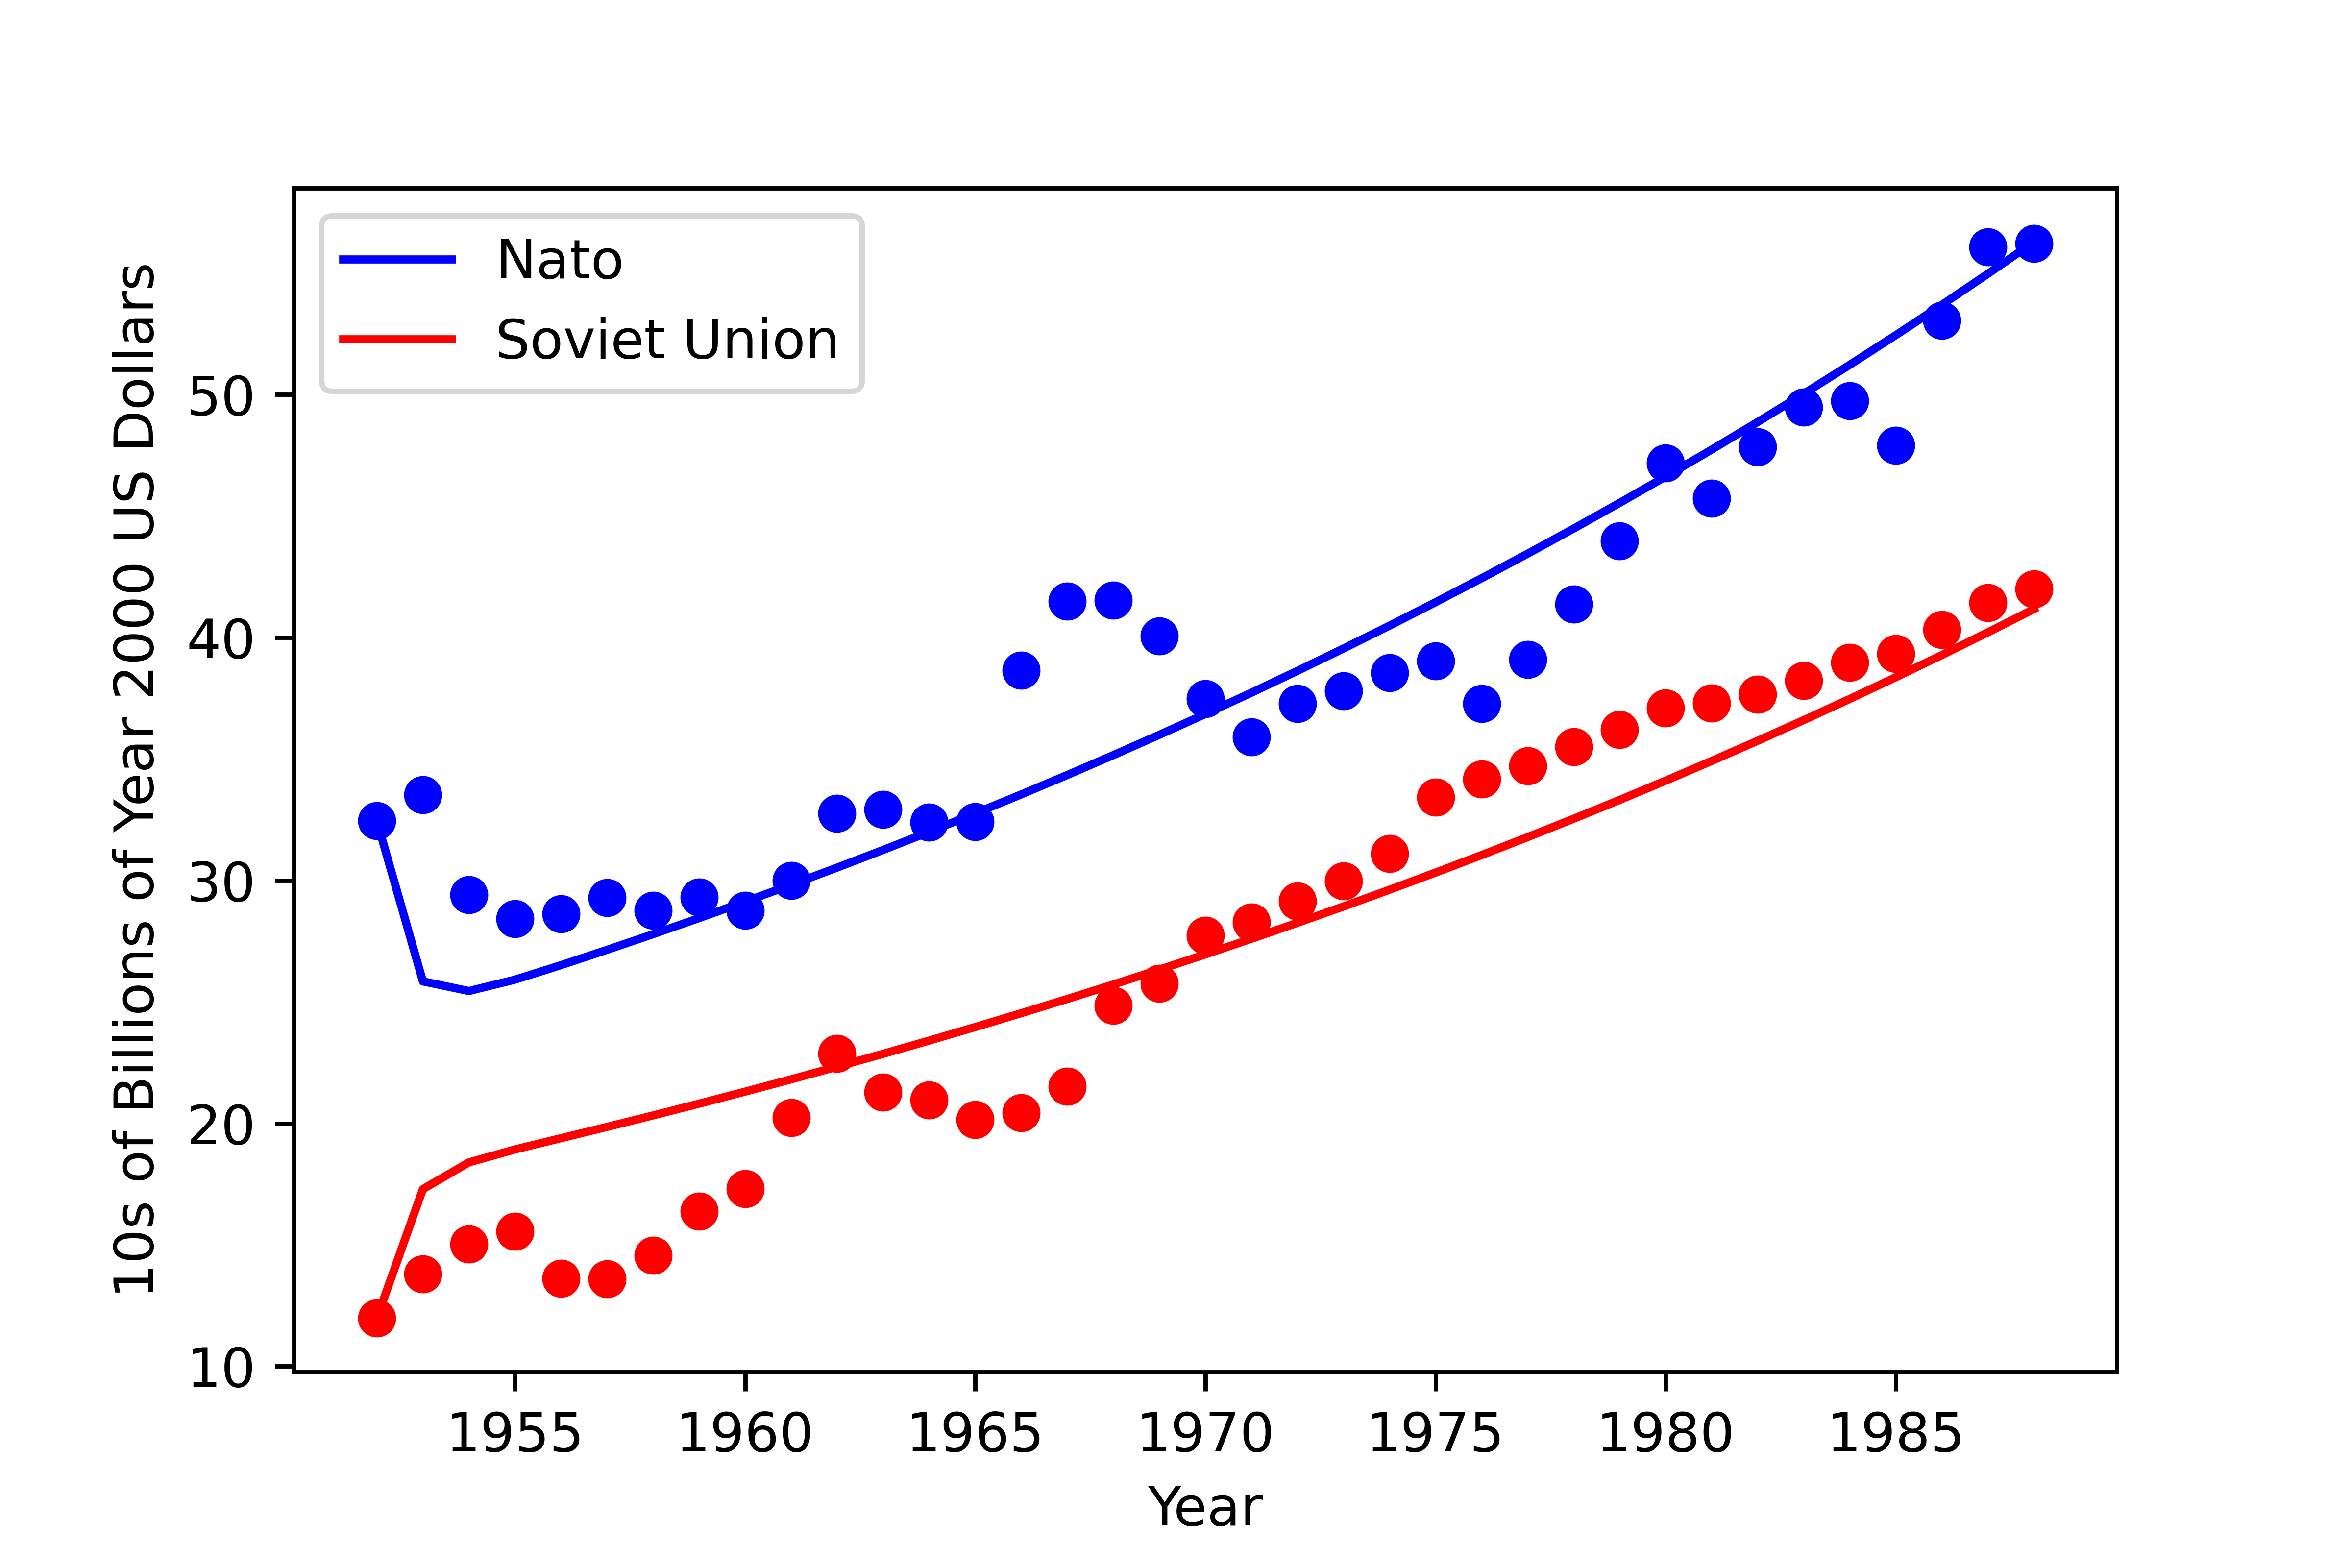
\includegraphics[width=8.25cm\textwidth]{NS2.png}\label{NS2}}
    \hfill
    \subfloat{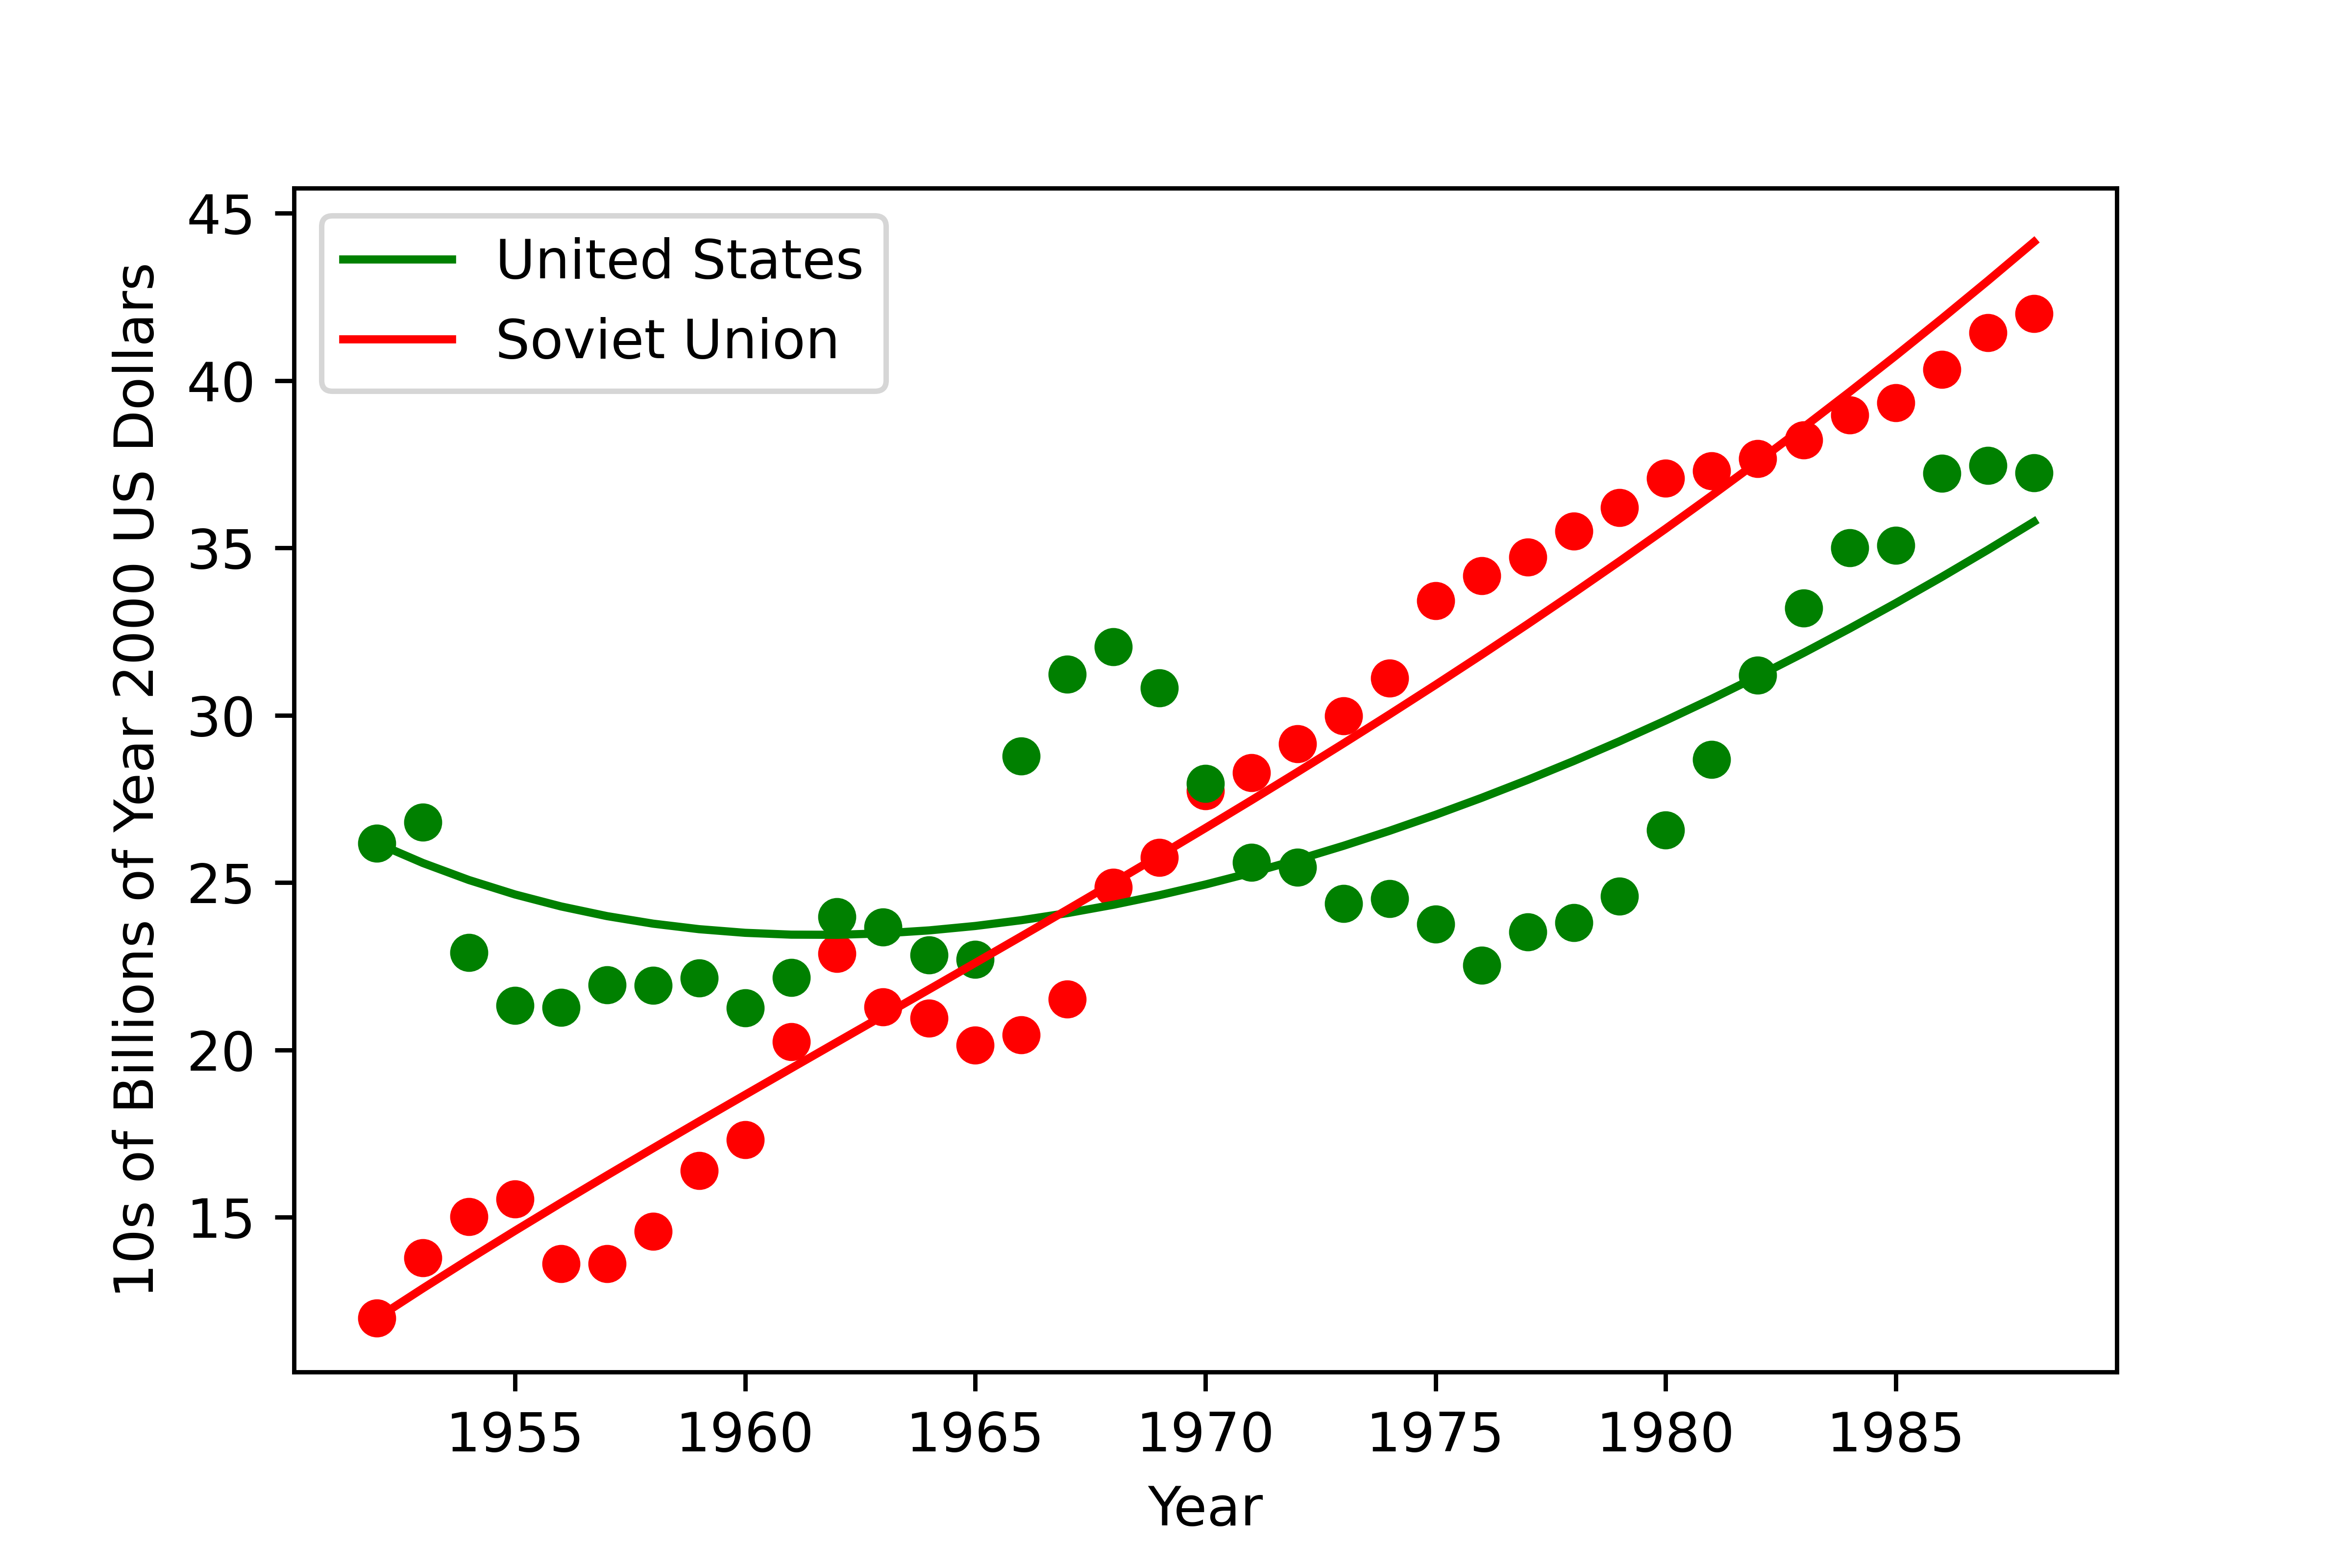
\includegraphics[width=8.25cm\textwidth]{US2.png}\label{US2}}
    \caption{Two Variable Richardson Model Fit}
\end{figure}
\squeezebit

The third simulation fits a model utilizing all variables of the Richardson Model including the fear factors, $a$ and $b$, the fatigue factors, $c$ and $d$, and the grievance factors between nations $i$ and $j$: $g_{ij}$. The resulting set of differential equations and models are 
\begin{equation*}\label{NS}
    \frac{dn}{dt}= as - cn + g_{ns} \quad ,\quad \frac{ds}{dt} = bn - ds + g_{sn}
\end{equation*}
\begin{equation*}\label{NS}
    \frac{du}{dt}= as - cu + g_{us} \quad ,\quad \frac{ds}{dt} = bu - ds + g_{su}
\end{equation*}
\squeezeup
%The resulting models fitting the data are 
\begin{figure}[htbp!]
    \centering
    \subfloat{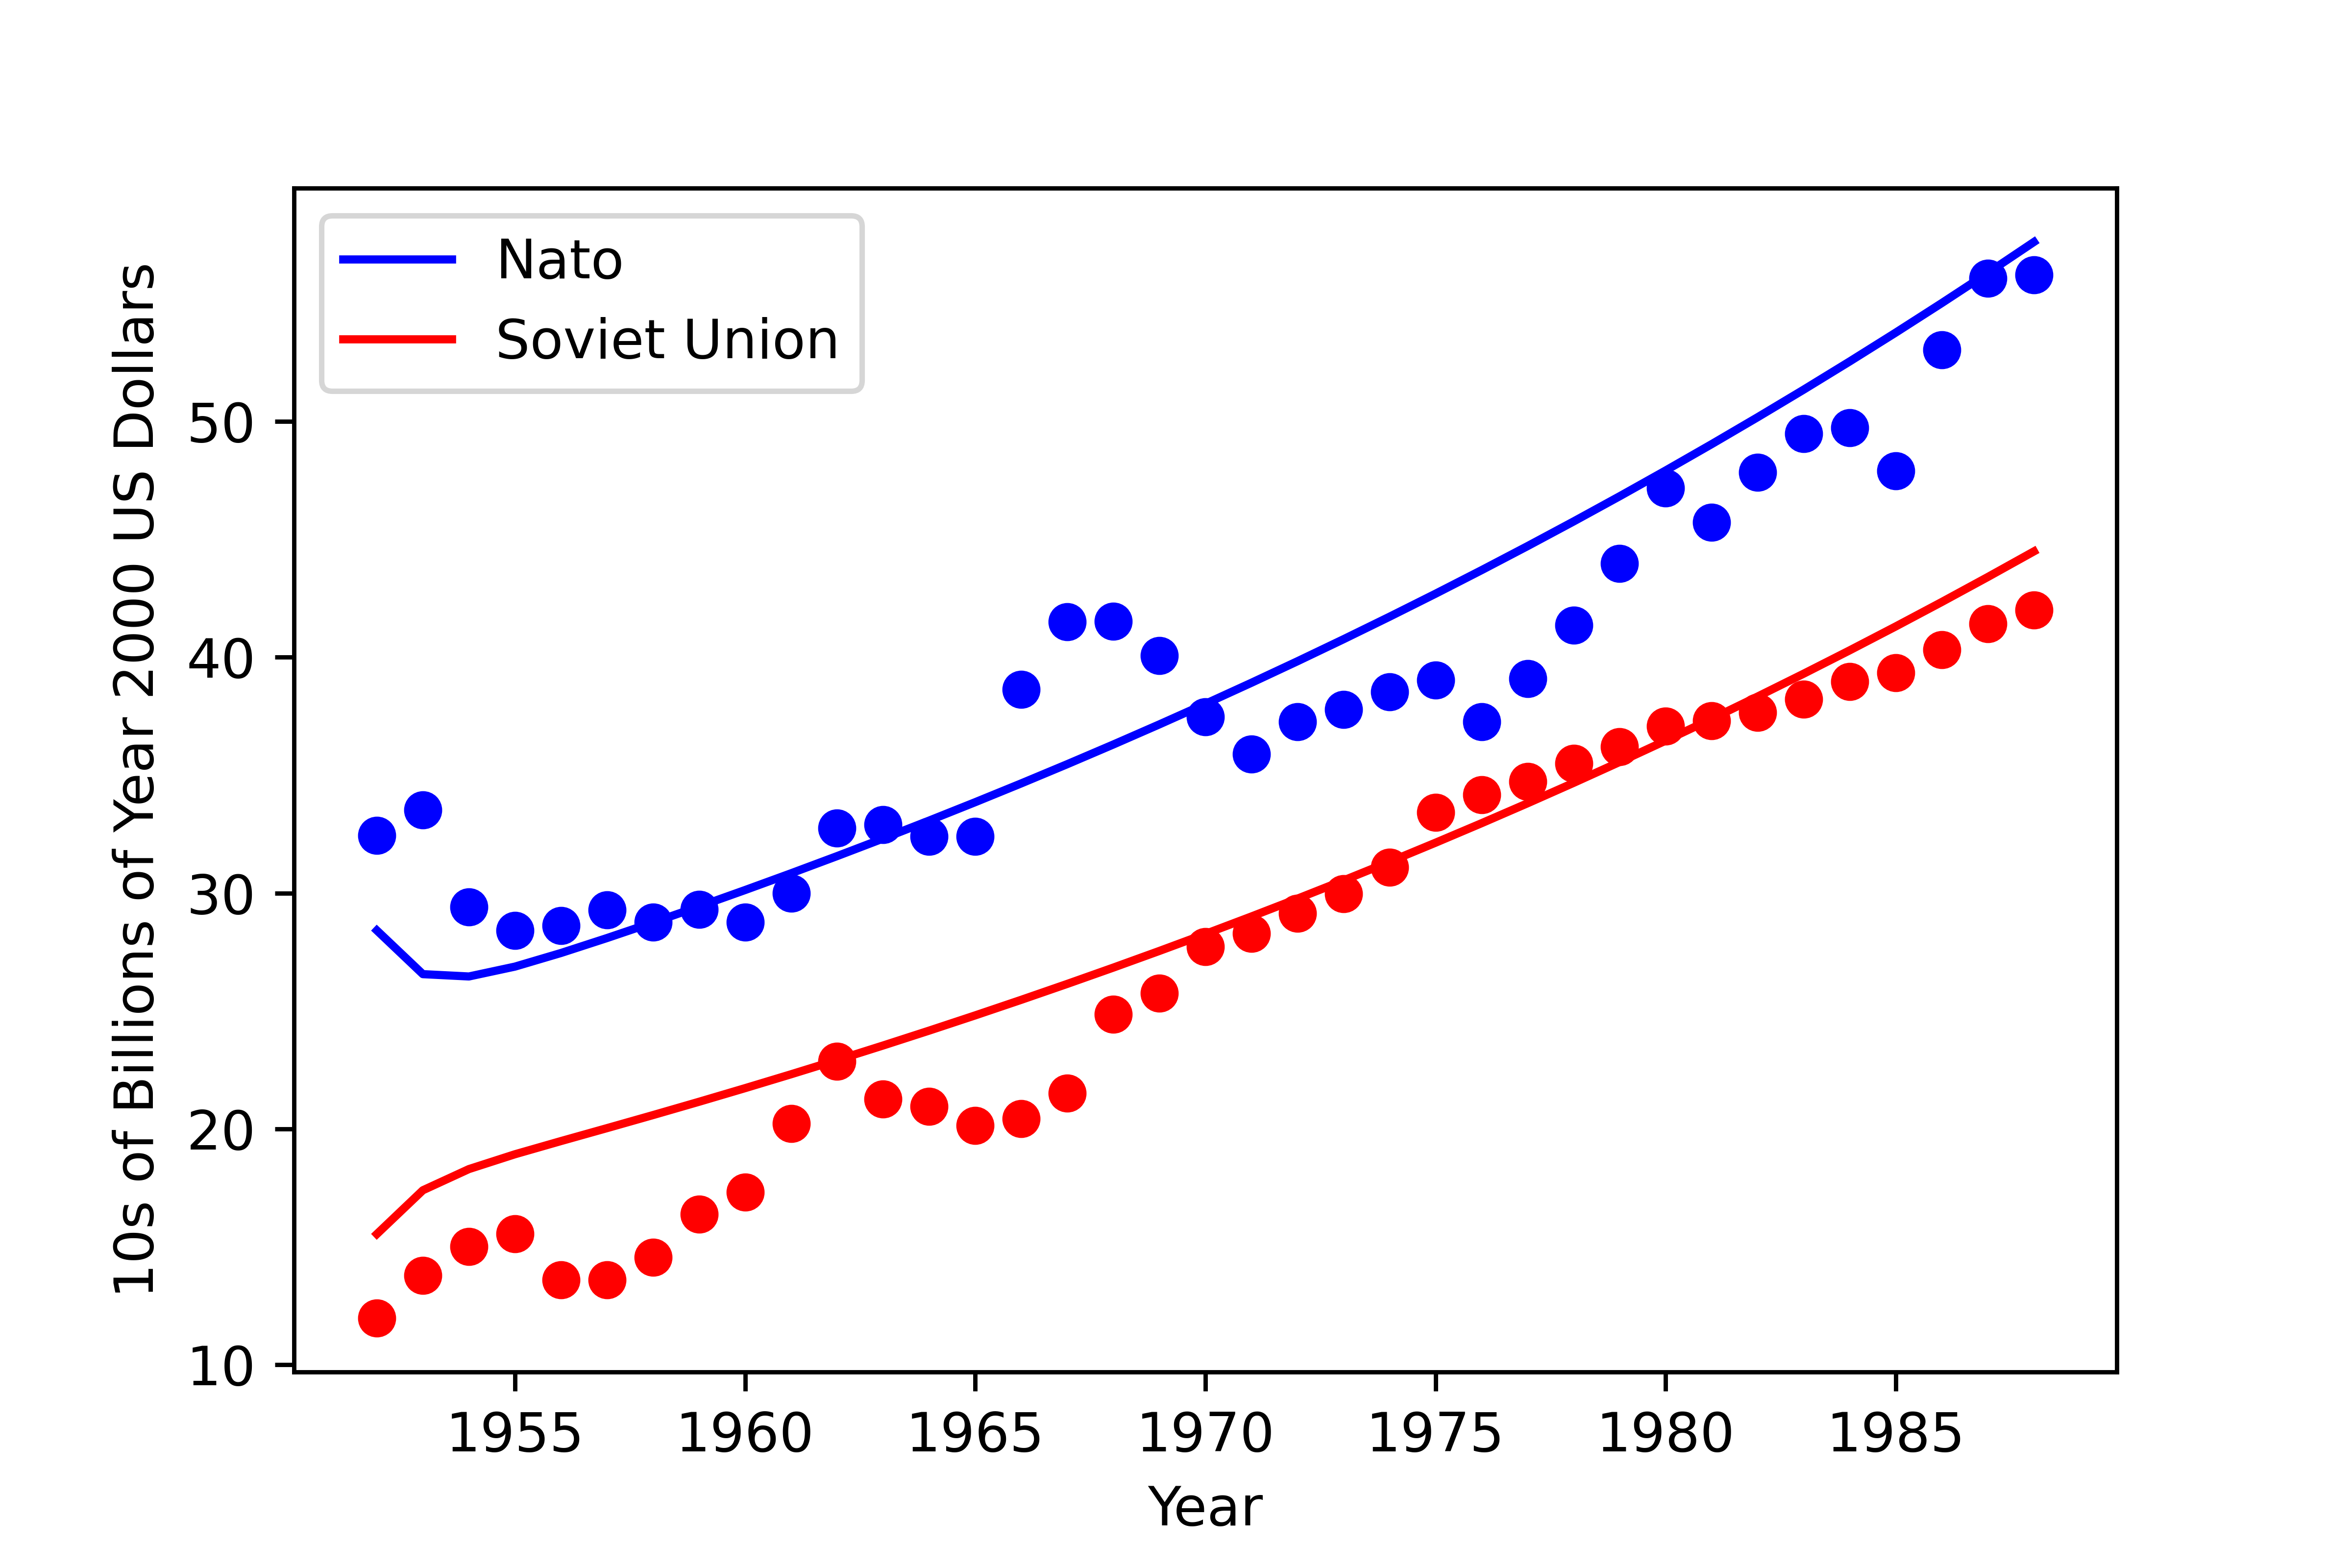
\includegraphics[width=8.25cm\textwidth]{NS3.png}\label{NS3}}
    \hfill
    \subfloat{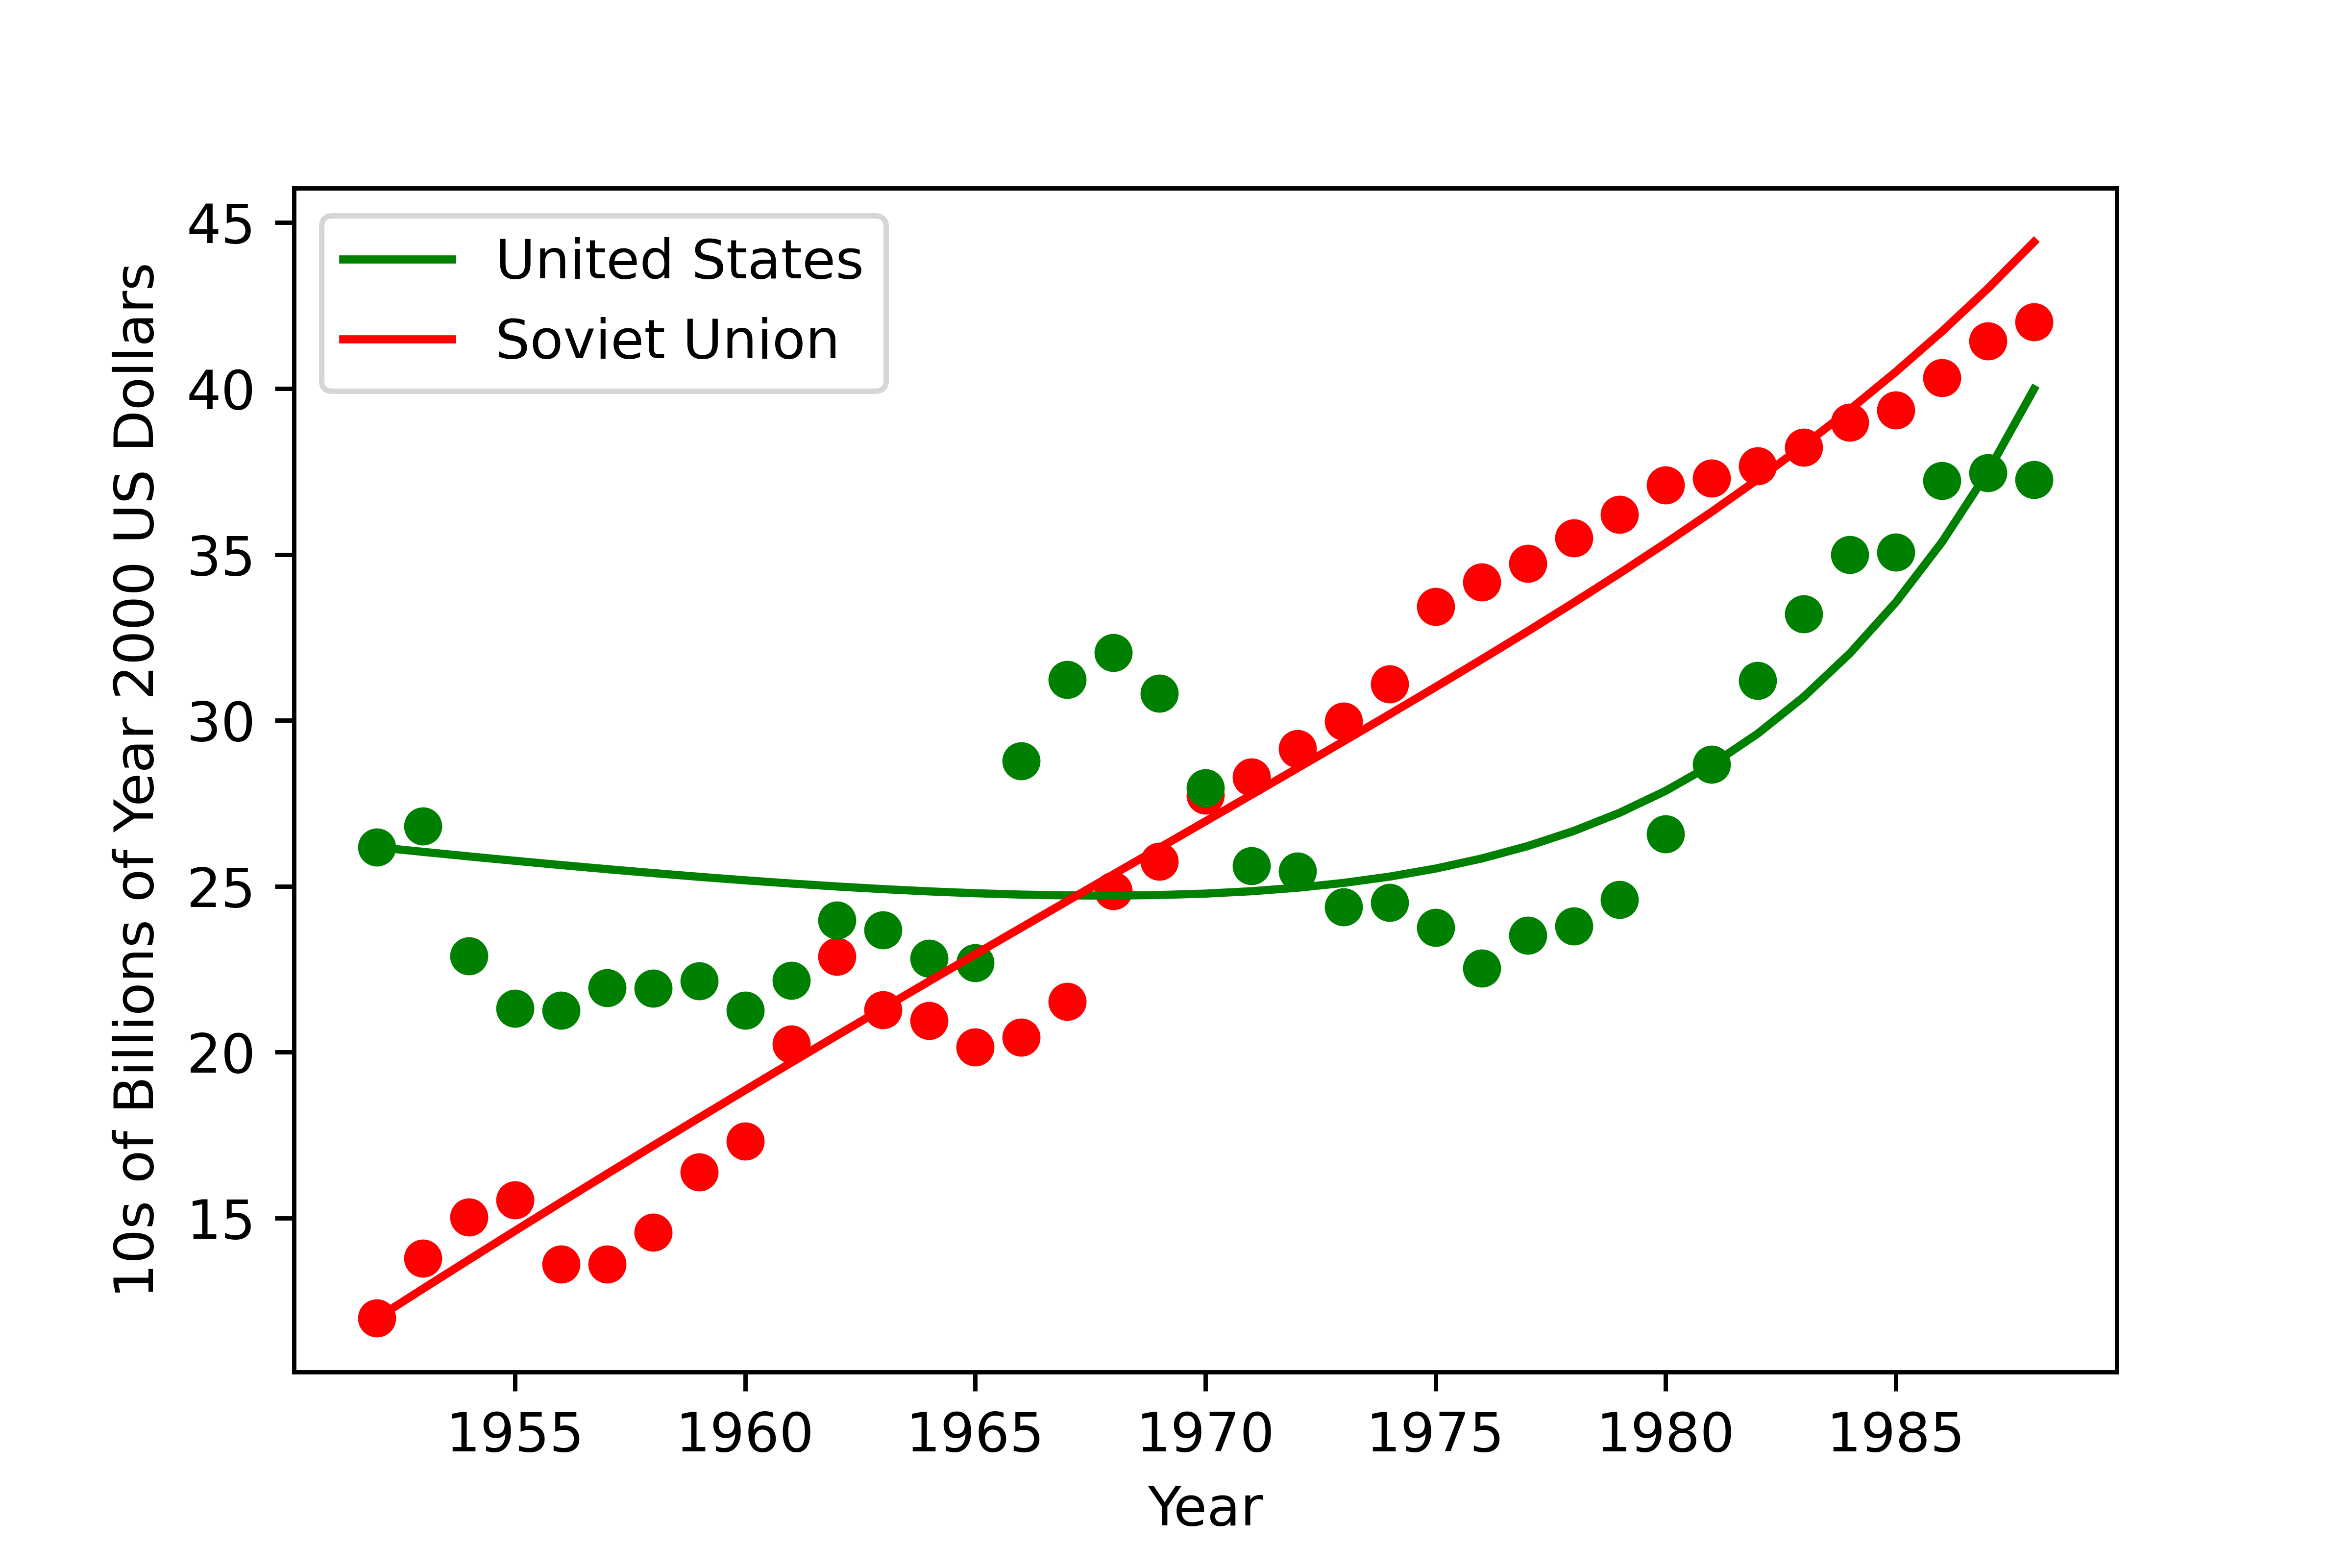
\includegraphics[width=8.25cm\textwidth]{US3.png}\label{US3}}
    \caption{Three Variable Richardson Model Fit}
\end{figure}
\newpage
Each of the model configurations produce lines of best fit for each country's military expenditure based on the minimization of the SSE between the lines of best fit and their respective data.

\begin{table}[htb!]
\centering{
\begin{tabular}{|l|c|c|}
\hline
\textbf{Model Configuration}     & \textbf{NATO \& USSR} & \textbf{USA \& USSR} \\
\Xhline{2\arrayrulewidth}
\textbf{One Variable}   & 549.45             & 742.32            \\
\hline
\textbf{Two Variable}   & 651.28             & 473.08            \\
\hline
\textbf{Three Variable} & 523.34             & 451.26
\\\hline
\end{tabular}
}
\caption{SSE's of Best-Fit Lines by Model Configuration (10s of Billions of Year 2000 USD)}
\label{sse}
\end{table}

By comparing the resulting plots and cumulative SSE's calculated, we conclude that the Richardson Model configuration utilizing all coefficients produces the lines of best fit with the smallest SSE. This is an expected result as the added coefficients allow for the representation of the limited resources of countries and the pre-existing grievances between countries. 

\subsection{Richardson Model Interpretation}

Utilizing the three-variable configuration of the Richardson Model, we seek to understand how the USSR would change their spending based on how both NATO and the United States of America changed their military expenditures. By halving both NATO and the United State's military expenditure increases from 1985 to 1990 the USSR's reactions to these decreases are shown. 

\begin{table}[htb!]
\centering{
\begin{tabular}{|l|c|c|}
\hline
\textbf{Change in Expenditure Increase}     & \textbf{NATO} & \textbf{USA} \\
\Xhline{2\arrayrulewidth}
\textbf{No Change}   & 17.99\%             & 13.22\%            \\
\hline
\textbf{50\% Reduction} & 5.44\%             &  -2.98\%
\\\hline
\end{tabular}
}
\caption{Percentage Change of USSR Military Expenditure from 1985 to 1990}
\label{results}
\end{table}
If NATO and the United States increased their expenditure normally, the USSR would continue to increase its expenditure. However, if the entities reduced the increase in their military expenditure, the USSR would still increase when reacting to NATO, but notably, it would decrease its expenditure when reacting to the United States.


%----------------------

\section{Conclusion}
% From our multiple models accounting for different factors, we can conclude that the three variable model is the best fit to our data. we can use the best model fit to then predict the spending up to 2007, where our data ends. Using the Richardson model, we can also infer that without the collapse of the Soviet Union, the arms race would have continued to potentially astronomical results. Continuing on for the next few years after our data ends with our three variable model, we find that expenditure would likely have started to increase at an exponential rate. These results ultimately would have lead to higher international tensions, and maybe even all out war. 

Based on the results of the simulation study, it is evident that the three variable Richardson Model fits best as it has the lowest cumulative SSE as seen in Table \ref{sse}. Furthermore, in Table \ref{results}, we show that a 50\% reduction military expenditure of the United States from 1985 to 1990 causes a contraction in overall military expenditure by the USSR. The USSR's reaction to a 50\% reduction by NATO was still an increase.  This suggests that the USSR's rate of military expenditure is more heavily influenced by the United State's expenditure than it is by NATO's. Understanding this, the disbandment of NATO and thereby reduction in spending in NATO would not have stopped the USSR from expanding its military presence; rather it would have simply grown at a slower rate. However, the models show that a reduction in the United State's military expenditure would not have caused the USSR to drastically expand its military. Instead, the USSR would have shrunk its military expenditure, slowing the Cold War arms race. Following the assumptive relationship between lower military expenditure and normalized relations made by \cite{solarin2018determinants}, a disbandment of NATO during the Cold War would have had little impact on global relations and international peace with the USSR. However, a reduction in the United States' growing military expenditure during the arms race would have resulted in more peaceful relations between the two nations. 

%Housing Prices: Future projections show this, from the model. Then write about what the future results indicate. 
%SIR Model: If you decrease the infection rate by 20\%, you will get a peak decrease of 15\%. 
%Sport Statistics: This model indicates player outcomes for this and this team to win these type of games. 
%This is half a page long. In Figure \ref{fig:bmi_xy}, we show the inputs for calculating body mass index.  As in \eqref{eq:simple_quad}, we have the formulation of a simple quadratic function. 

%----------------------

%This is an example reference \cite{pocuca2020}, 

%Defying circadian rhythm leads to adverse effects \citep{pocuca2020}. 

%Defying circadian rhythm leads to adverse effects as shown in \cite{pocuca2020}. 

\newpage
\bibliographystyle{chicago}
\bibliography{BIB}

%----------------------

\newpage
\section*{Appendix}
\subsection{Coefficient Optimization Tolerance}
For all optimization utilizing the \texttt{SciPy} Python module \citep{2020SciPy-NMeth}, the tolerance setting is set to \texttt{tol = 1e-5}.

\subsection{Processed Data Plot}
The scatter plot of the data after processing is plotted as
\begin{figure}[!htb]
    \centering
    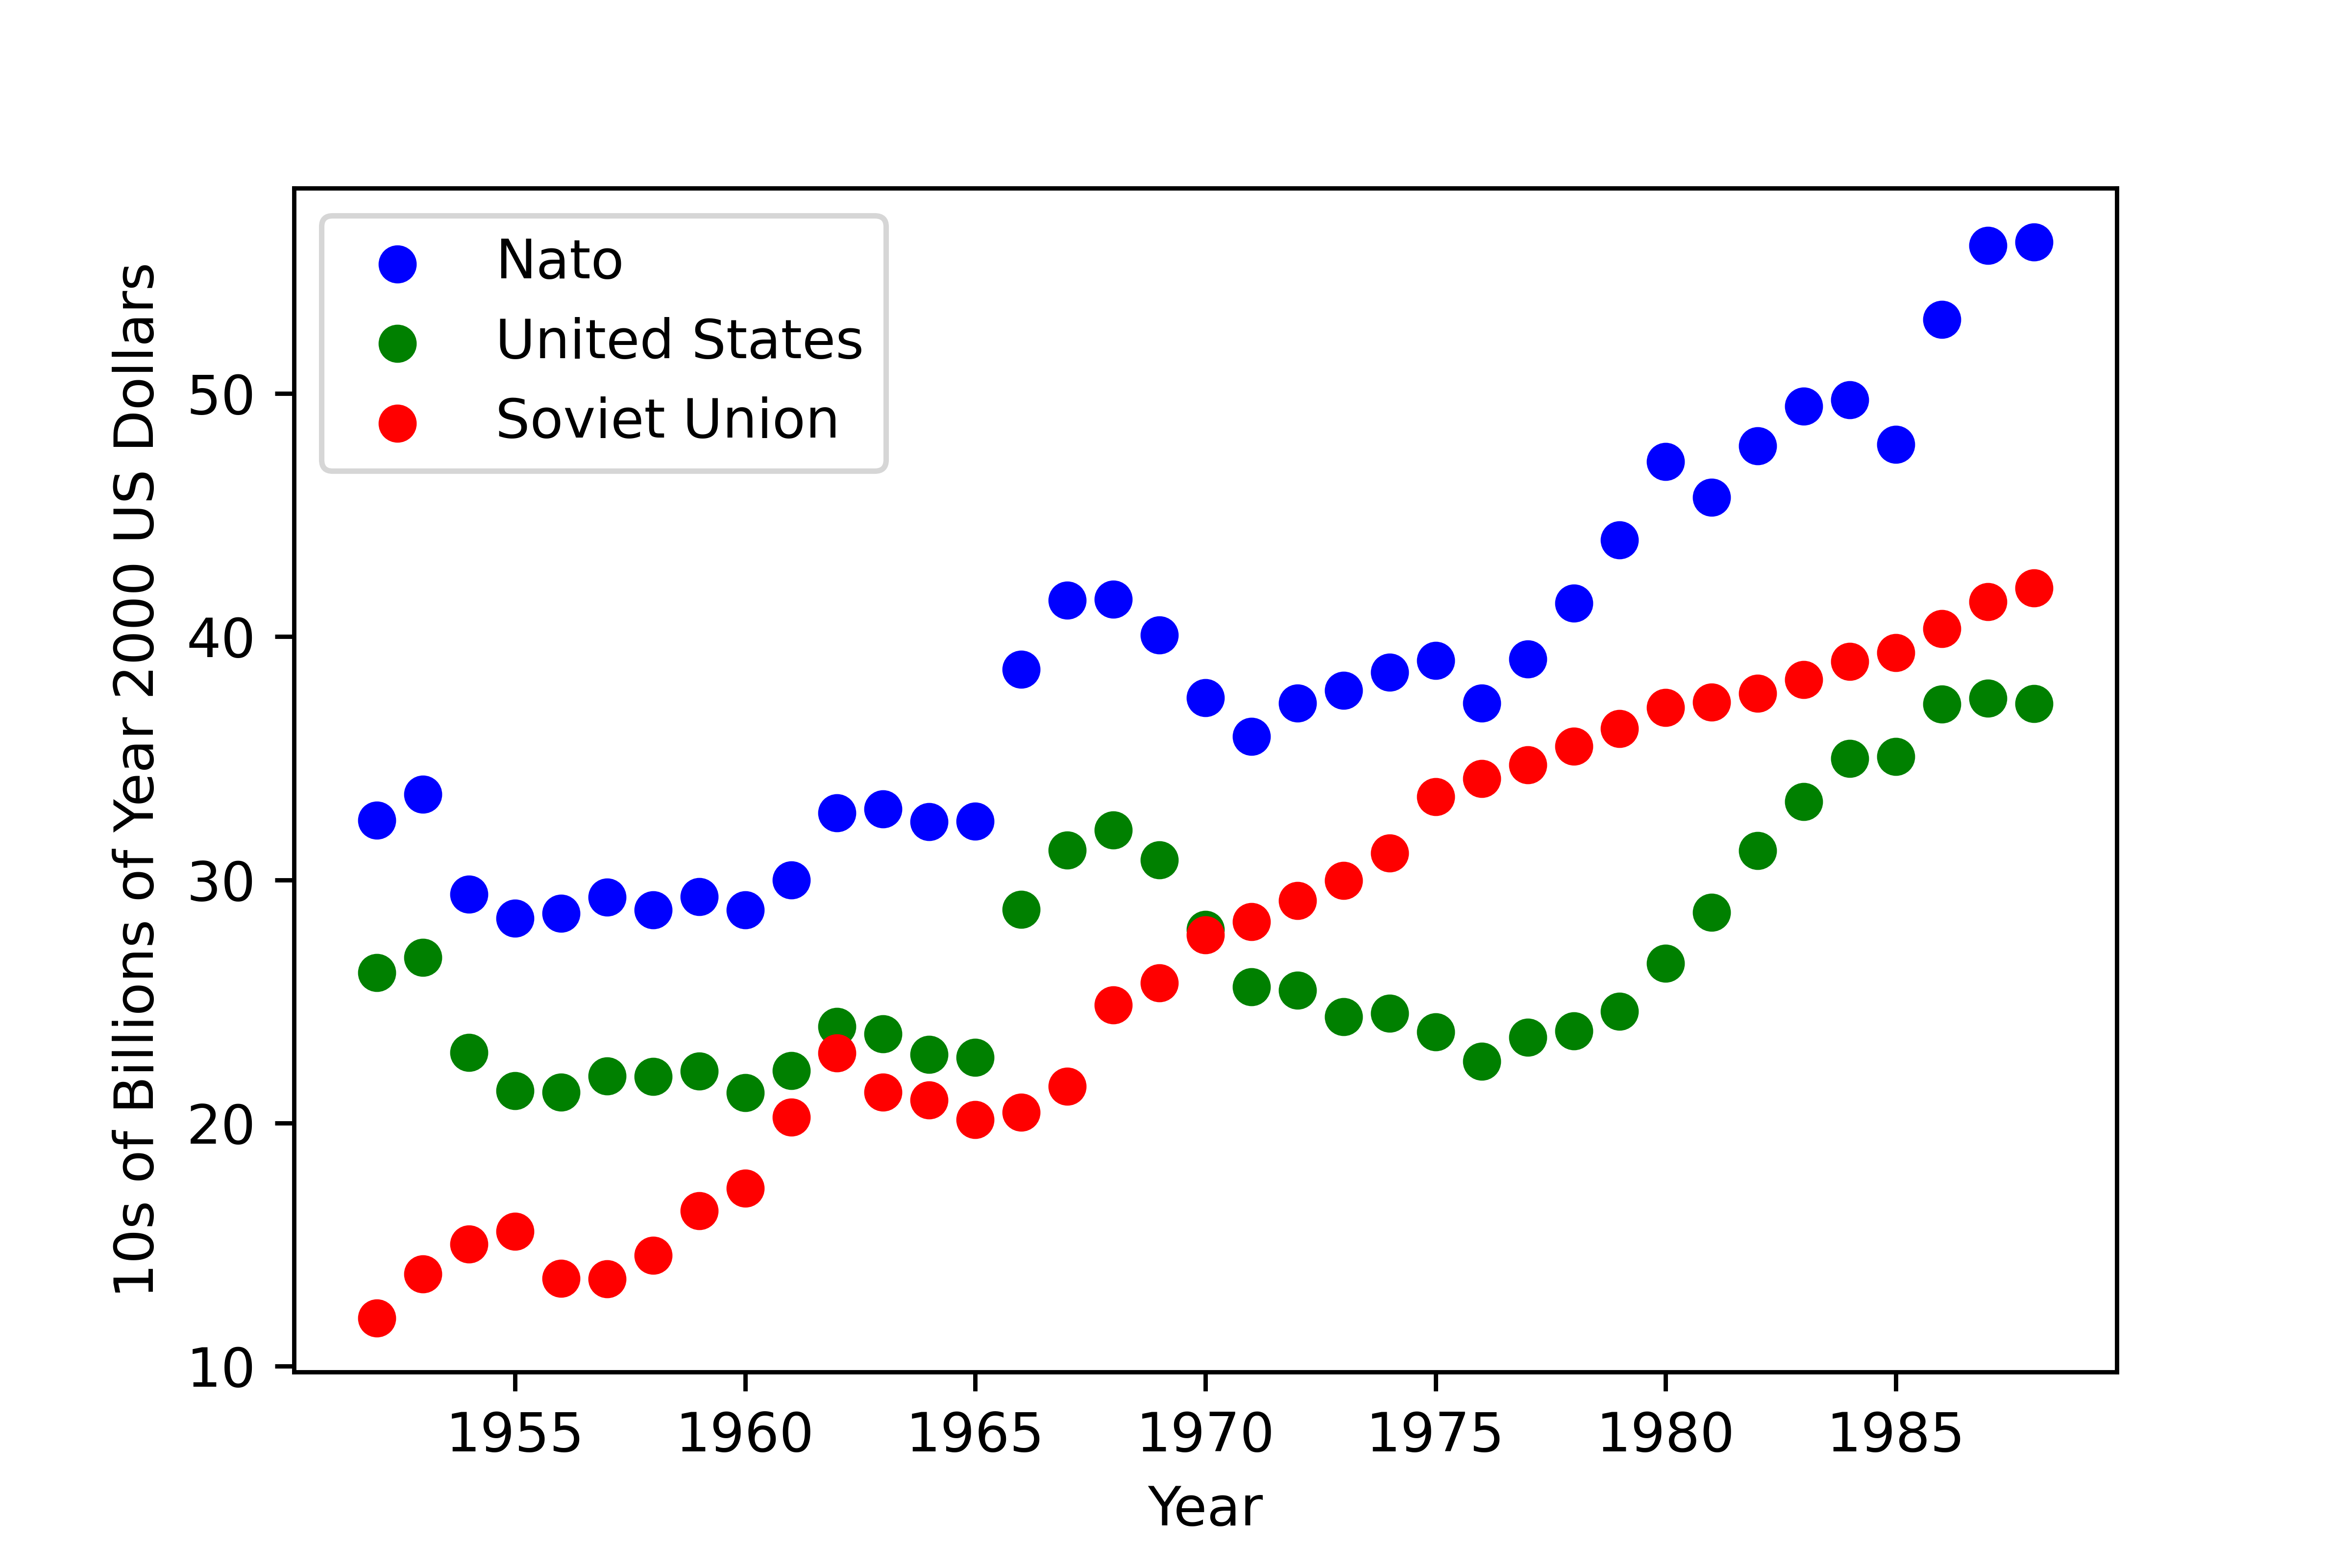
\includegraphics[width=10cm]{NUS0.png}
    \caption{Country Military Expenditure Data by Year}
    \label{fig:data}
\end{figure}

\end{document}